% !TeX root = ./main.tex
\documentclass[12pt, a4paper]{report}

%encoding
%--------------------------------------
\usepackage[T1]{fontenc}
\usepackage[utf8]{inputenc}
%--------------------------------------

%Portuguese-specific commands
%--------------------------------------
\usepackage[portuguese]{babel}
%-------

%Packages
%--------------------------------------
\usepackage{hyperref}
\usepackage{import}
\usepackage{graphics}
\usepackage{graphicx}
\usepackage{float}
%-------

%---------------------------------------
% -------------- Config ----------------
%---------------------------------------

% Glossaries
%--------------------------------------
\usepackage[acronym]{glossaries}
\makeglossaries{}

\newacronym{bu}{BU}{Business Unit}
\newacronym{iaas}{IaaS}{Infrastructure as a Service}
\newacronym{iac}{IaC}{Infrastructure as Code}
\newacronym{aws}{AWS}{Amazon Web Services, Inc.}
%-------

%Declare assets
%--------------------------------------
\graphicspath{{../assets/}}
%-------

%--------------------------------------
%begin document
\begin{document}
\pagenumbering{gobble}

\title{Documentação Geral de Infraestrutura em Nuvem Pública da Plataforma SociaLab}
\author{SociaLab, ZRP}
\date{\today}


\maketitle{}

\begin{abstract}
	Com base em consultas à usuários e operadores da plataforma SociaLab, percebe-se que existem desafios técnicos, operacionais e de negócios significativos para o desenvolvimento e implantação de de uma infraestrutura em nuvem. Estes incluem, mas não estão limitados ao seguinte: Falta de conhecimento técnico e operacional para sustentação contínua da plataforma, ausência de fluxo ágil no desenvolvimento de novas funcionalidades e seu lançamento, irreplicabilidade do processo de construção da infraestrutura e ausência de documentação.

	Com base nisso, o presente trabalho aborda infraestrutura através do conceito de \acrlong{iac} (\acrshort{iac}), que representa de forma abstrata como componentes virtuais de software e hardware estão relacionados, para tal utilizando um conjunto de módulos que expõe as capacidades, recursos, interfaces, entradas e saídas necessárias à sustentação da aplicação e de seus periféricos. Apoiado na representação abstrata, diferentes provedores de nuvem podem ser utilizados para a construção da mesma infraestrutura, partindo do princípio de \acrlong{iaas} (\acrshort{iaas}).

	O documento começa a partir do resumo e, à medida que avança, vai entrando cada vez mais em detalhes. Ele segue o processo de design tradicional de infraestrutura, onde você começa com os princípios básicos, avança para conceitos e modelos abstratos e termina com considerações operacionais, como segurança e gerenciamento do ciclo de vida da infraestrutura.

	Este documento foi desenvolvido pela ZRP, para mais informações, consulte \url{https://zrp.com.br}.
\end{abstract}

\pagenumbering{arabic}

\tableofcontents{}
\listoftables
\listoffigures
\printglossary{}

\printglossary[type=\acronymtype]

\chapter{Arquitetura}

\paragraph{
	A arquitetura delimita os blocos básicos de construção da infraestrutura. Entende-se infraestrutura, no presente documento, como o conjunto \(S\) de recursos em nuvem necessários à implementação concreta de um módulo. Embora existam elementos na arquitetura que se relacionam intimamente às capacidades de um provedor, nela estipulam-se primordialmente o conjunto de módulos abstratos necessários ao funcionamento da infraestrutura, sendo assim, neste capítulo, abordados tanto aspectos gerais dos módulos, bem como aspectos específicos do provedor selecionado (\acrshort{aws}).
}

\section{Estrutura Geral}

Adicionalmente aos problemas organizacionais e de negócio apresentados, observa-se na arquitetura presente problemas também ligados a sua implementação, sendo notáveis (mas não apenas os únicos):

\begin{itemize}
	\item Regiões físicas diferentes de deploy (notadamente us-east-1 e us-west-2);
	\item Arquitetura baseada em serviços em rede pública;
	\item Ambiente estático, não replicável e não redundante;
	\item Falta de gestão a nível organizacional de diferentes ambientes;
	\item Falta de múltiplos ambientes para homologação dos serviços disponíveis ao consumidor.
\end{itemize}

\newpage

Face aos problemas apresentados, a arquitetura proposta têm por objetivos:

\begin{itemize}
	\item Melhorar a performance geral da aplicação;
	\item Prover métricas e logs de sistema a nível de infraestrutura;
	\item Inibir o acesso irrestrito a informações sensíveis;
	\item Automatizar a gestão de recursos e escalabilidade da aplicação.
	\item Permitir a replicação fácil e rápida dos recursos de infraestrutura e da aplicação;
	\item Garantir segurança operacional, redundância e backup da informação;
	\item Múltiplos ambientes com diferentes finalidades (homologação, teste, desenvolvimento, produção).
\end{itemize}

Para atingir tais objetivos, a arquitetura foi então desenhada compartimentando as diferentes responsabilidades que a aplicação possui em módulos, sendo estes módulos: Rede, Dados, Serviços, Segurança e Roteamento.

\begin{center}
	\begin{figure}[H]
		\noindent\makebox[\linewidth]{
			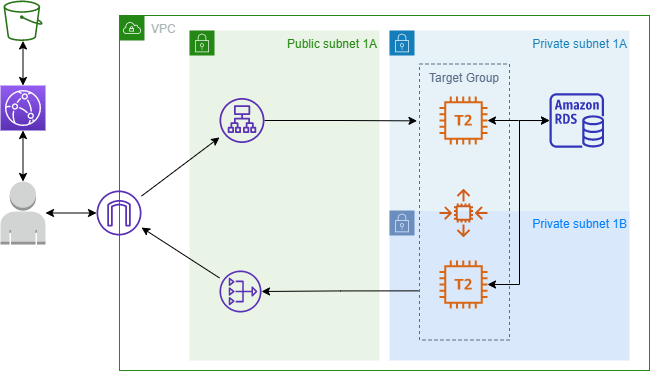
\includegraphics[width=\linewidth,keepaspectratio]{01-overview.png}
		}
		\caption{Fluxo de requisição de usuário da plataforma}\label{fig:01-overview}
	\end{figure}
\end{center}

\section{Convenções}

Neste capítulo são abordadas as principais convenções adotadas na confecção da infraestrutura em nuvem, bem como os aspectos organizacionais envolvidos e a melhor forma de gerenciá-los.

\subsection{AWS Organizations}

A organização é a macroestrutura responsável pela gestão de uma ou mais contas em nuvem, podendo diferentes contas corresponderem à áreas ou \acrshort{bu}'s (\acrlong{bu}).

\subsection{Tags}

As tags permitem organizar recursos da infraestrutura e elementos organizacionais adjacentes.

Isso permite um controle e visão mais granulares desses recursos, como custo, além de permitir a remoção de múltiplos elementos de uma única vez, ou clarificar os responsáveis por um recurso ou organizações associadas ao recurso.

Dado isso, as tags são separadas da seguinte forma:

% \begin{table}
% 	\begin{center}
% 		\begin{tabular}{ |c|c|c|c| }
% 			\hline
% 			col1 & col2 & col3 \\
% 			\hline
% 		\end{tabular}
% 	\end{center}
% 	\caption{Exemplo}\label{table:1}
% \end{table}

A estrutura das tags segue por princípio a seguinte estrutura:

prefixo, contexto, identificador, ex.socialab:application:id
que identifica a qual aplicação a infraestrutura atual se referencia.

\section{Provedor de IaC}
\section{Replicabilidade}
\section{Segurança}
\chapter{Módulos}

\section{Rede}
\section{Interface}
\section{Servidores}
\section{Serviços}
\section{Dados}

\chapter{Operação}

\section{Manutenção de Estado}
\section{Atualização de Estado}
\section{Acesso e Controle}
\section{Custos}

\end{document}
